\subsection{Use Case 4: Place Ad}

\subsubsection{General Description}

\begin{tabular}{|p{.2\linewidth}|p{.65\linewidth}|}
\hline 
ID: & place ad \\ \hline
Goal: & To enable the promotion of an medical professional, consequently making revenue \\ \hline
Precondition: & A verified advertiser payed for an ad placement \\ \hline
Postcondition: & Advertisements are shown to the user as long as the advertiser pays for it. \\ \hline
Involved Users: & Advertiser: Someone who is verified and has the means to advertise \\ \hline
\end{tabular}

\subsubsection{UI to call the use case}

\begin{center}
\begin{figure}[H]
\centering
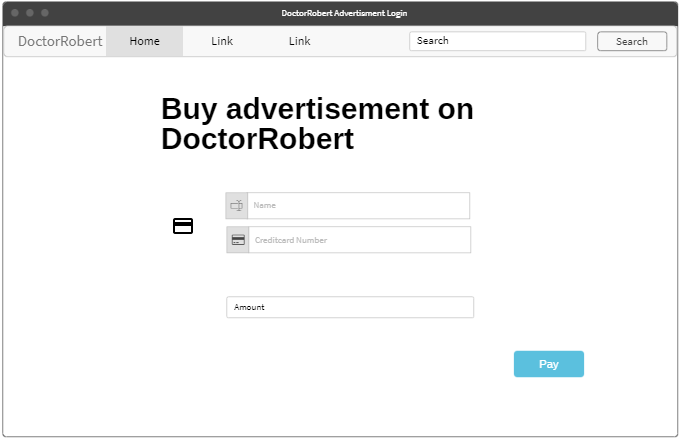
\includegraphics[scale=0.8]{SystemSpec/Usecases/Mocks/placead01.PNG}
\caption{\label{fig:blue_rectangle}Place Ad}
\end{figure}
\end{center}

The advertiser can choose between multiple payment methods. The payment itself will be outsourced to Stripe and PayPal.

\subsubsection{The Standard Use}

If a user is an verified advertiser, he will have the option place advertisements in our app via our website. To place ads the advertiser has to pay us. The amount paid will determine how frequent and how often the ads will be shown. Similar to Google's advertisement model an advertiser pays for one ad and for every time the ad is shown we will charge a small fee and after the whole amount is used the ad will no longer be shown on our app. An appropriate message to inform the advertiser will be sent. One can find an corresponding illustration in the subsection \hyperlink{AdIllustration}{2.4 Use Case 2: Get Diagnosis}



\subsubsection{The Non-Standard Use}

\begin{itemize}
    \item The payment doesn't go through
    
    If the payment doesn't go through, because for example they entered wrong payment information or a trying to scam us, we simply will not show the ad and send the advertiser a rejection message.
    
\end{itemize}

\pagebreak
